\chapter{Étude et préparation des données}
\label{chap:donnees}

\section{Introduction}

La qualité d'un modèle de Machine Learning dépend en grande partie des données sur lesquelles il est entraîné. Avant tout apprentissage, il est donc indispensable de choisir un \textbf{jeu de données adapté}, d'en comprendre la composition et de le préparer avec rigueur. Ce chapitre présente l'étude des datasets disponibles, la justification de notre choix, l'analyse quantitative et qualitative des données retenues, puis les différentes étapes de préparation : nettoyage, redimensionnement, normalisation et séparation en jeux d'entraînement, de validation et de test.

\section{Étude des datasets disponibles}

Plusieurs jeux de données publics ont été étudiés afin de trouver celui qui répond le mieux aux besoins du projet.

\begin{table}[H]
\centering
\small
\caption{Comparaison des datasets étudiés}
\begin{tabularx}{\textwidth}{>{\raggedright\arraybackslash}p{3.2cm}>{\raggedright\arraybackslash}p{2.2cm}YY}
  \toprule
  \entete \textbf{Dataset} & \textbf{Classes couvertes} & \textbf{Atouts} & \textbf{Limites} \\
  \midrule
  \href{https://cocodataset.org/\#download}{COCO 2017} & Les 6 & Photos réelles, une boîte annotée par objet & Fort déséquilibre, nombreux petits objets, recadrages à réaliser \\
  CIFAR-10 et CIFAR-100 & Les 6, en combinant les deux & Téléchargement simple, images déjà centrées & Images de 32~×~32~px seulement, peu de scènes routières \\
  Pascal VOC 2012 & 5 sur 6 & Annotations soignées, taille raisonnable & Absence de la classe camion \\
  Jeux Kaggle \og véhicules \fg{} & Variable & Prêts à l'emploi & Qualité et licences inégales, souvent sans personne ni vélo \\
  \bottomrule
\end{tabularx}
\end{table}

\section{Comparaison et justification du dataset retenu}

Le descriptif du projet laisse le choix du jeu de données à l'équipe, en demandant seulement qu'il contienne des images d'objets routiers. Pour départager les options étudiées, nous avons défini cinq critères, directement liés aux besoins du projet :

\begin{itemize}
  \item \textbf{Couverture des classes}\\
  Le dataset doit contenir les six classes retenues, sans devoir en abandonner une.
  \item \textbf{Réalisme des images}\\
  Les photos doivent montrer des objets dans des situations réelles et variées, proches de ce que verrait un véhicule.
  \item \textbf{Résolution suffisante}\\
  Les objets doivent rester reconnaissables une fois recadrés, ce qui exclut les images trop petites.
  \item \textbf{Annotations par objet}\\
  Chaque objet doit être localisé par une boîte, afin de pouvoir le découper automatiquement.
  \item \textbf{Licence et documentation}\\
  Le dataset doit être documenté, cité dans la littérature et utilisable dans un cadre scolaire.
\end{itemize}

\begin{table}[H]
\centering
\small
\caption{Comparaison des datasets selon nos critères}
\begin{tabularx}{\textwidth}{>{\raggedright\arraybackslash}p{3.1cm}YYYY}
  \toprule
  \entete \textbf{Critère} & \textbf{COCO 2017} & \textbf{CIFAR-10/100} & \textbf{Pascal VOC} & \textbf{Kaggle} \\
  \midrule
  Couverture des 6 classes & Oui & Oui, en combinant les deux & Non (5 sur 6) & Variable \\
  Réalisme des images & Oui, scènes réelles variées & Faible, objets isolés & Oui & Variable \\
  Résolution & Médiane de 640~×~480~px & 32~×~32~px & Correcte & Variable \\
  Annotations par objet & Oui, boîtes englobantes & Non, une étiquette par image & Oui & Variable \\
  Documentation et licence & Article de référence, licences précisées & Documenté & Documenté & Inégales \\
  \bottomrule
\end{tabularx}
\end{table}

Au regard de ces critères, nous avons retenu \textbf{COCO 2017}, sous réserve de la validation de notre encadrante. Il s'agit du seul dataset étudié qui remplit l'ensemble des critères : il couvre nos six classes avec de \textbf{vraies photos}, prises dans des conditions variées, et fournit des \textbf{annotations de référence} pour chaque objet. De plus, il n'est pas nécessaire de télécharger les 18~Go d'images, puisque seules les photos utiles sont récupérées grâce à leur adresse. CIFAR reste notre solution de secours, malgré sa résolution très faible.

\subsection{Source et description du dataset retenu}

\begin{table}[H]
\centering
\small
\caption{Fiche descriptive du dataset COCO 2017}
\begin{tabularx}{\textwidth}{>{\raggedright\arraybackslash}p{3.6cm}Y}
  \toprule
  \entete \textbf{Élément} & \textbf{Description} \\
  \midrule
  Nom & COCO (\textit{Common Objects in Context}), version 2017 \\
  Auteurs & Microsoft et plusieurs équipes universitaires, publication de référence de Lin et al. (2014) \cite{coco} \\
  Source & Site officiel \url{https://cocodataset.org}, rubrique \textit{Download} \\
  Contenu & 80 catégories d'objets du quotidien, dont nos six classes \\
  Volume & 118~287 images d'entraînement (\texttt{train2017}) et 5~000 images de validation (\texttt{val2017}) \\
  Annotations & Fichiers JSON : catégorie, boîte englobante et indicateur de foule pour chaque objet \\
  Licences & Annotations sous licence CC~BY~4.0, images sous la licence Flickr choisie par chaque auteur \\
  Utilisation dans le projet & \texttt{train2017} pour constituer nos jeux d'entraînement, de validation et de test, et \texttt{val2017} réservé aux tests sur de nouvelles images \\
  \bottomrule
\end{tabularx}
\end{table}

Concrètement, nous téléchargeons d'abord le fichier d'annotations de \texttt{train2017}, qui décrit chaque objet sans contenir les images. Nous sélectionnons ensuite les objets utiles, puis nous téléchargeons uniquement les photos correspondantes à partir de leur adresse. Les licences imposent de citer COCO et de ne pas redistribuer les images : celles-ci restent donc hors du dépôt Git, qui ne conserve que de petites vignettes dans les figures.

\section{Présentation des classes}

Les six classes retenues correspondent aux usagers de la route que le véhicule doit savoir reconnaître :

\begin{itemize}
  \item \textbf{Personne (\texttt{person})}\\
  Il s'agit de l'usager le plus vulnérable. Une erreur sur cette classe est donc la plus grave pour un véhicule.
  \item \textbf{Vélo (\texttt{bicycle})}\\
  Usager lent et fragile, souvent accompagné d'une personne. Il faut noter que COCO annote le vélo et non le cycliste.
  \item \textbf{Voiture (\texttt{car})}\\
  Usager le plus fréquent, souvent à l'arrêt sur la chaussée.
  \item \textbf{Moto (\texttt{motorcycle})}\\
  Véhicule léger et rapide, visuellement proche du vélo.
  \item \textbf{Bus (\texttt{bus})}\\
  Grand véhicule qui masque une partie de la visibilité.
  \item \textbf{Camion (\texttt{truck})}\\
  Grand véhicule. COCO range également dans cette classe des pick-ups et des camionnettes.
\end{itemize}

L'ordre des classes (personne, vélo, voiture, moto, bus, camion) est fixé une fois pour toutes, car il correspond aux sorties du modèle et à ce qu'attend le simulateur.

\begin{figure}[H]
  \centering
  \begin{subfigure}[t]{0.155\textwidth}\centering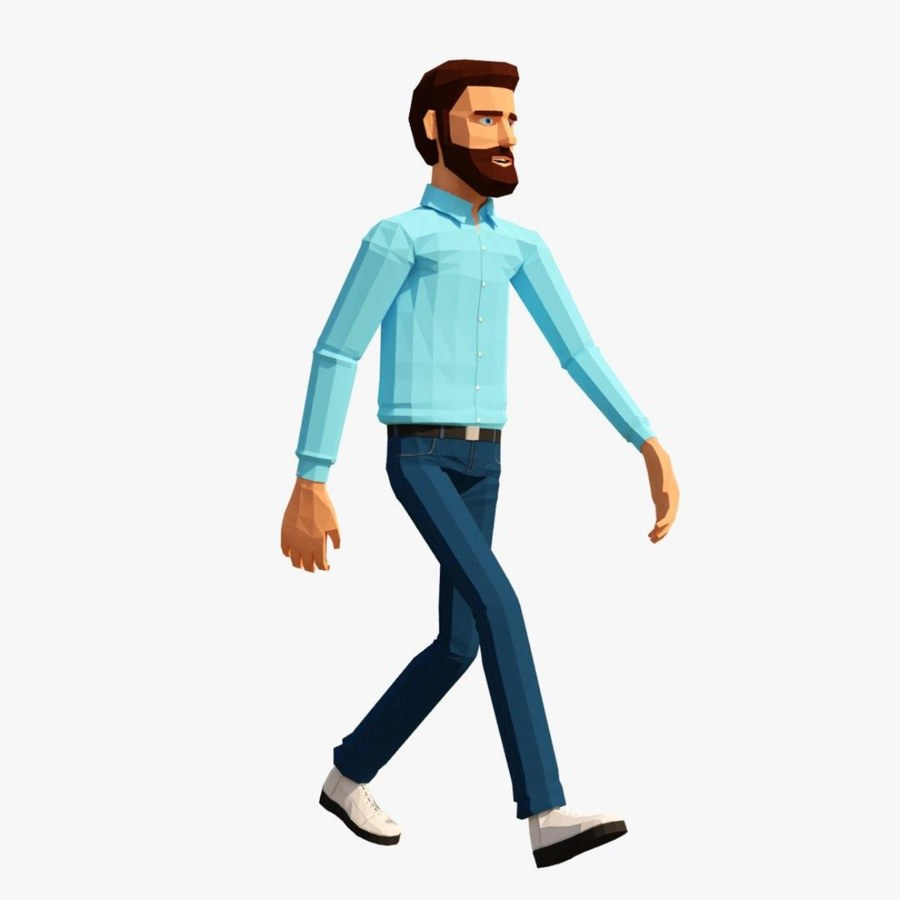
\includegraphics[width=\textwidth,height=2.6cm,keepaspectratio]{obj_person.jpg}\caption*{Personne}\end{subfigure}\hfill
  \begin{subfigure}[t]{0.155\textwidth}\centering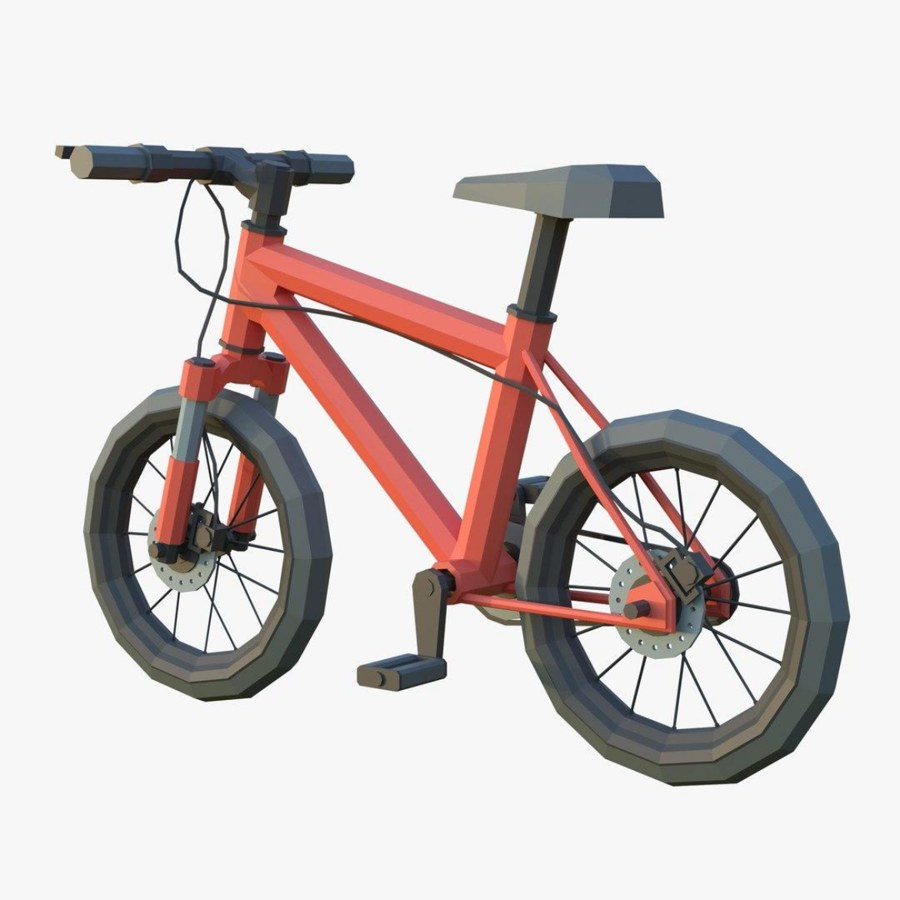
\includegraphics[width=\textwidth,height=2.6cm,keepaspectratio]{obj_velo.jpg}\caption*{Vélo}\end{subfigure}\hfill
  \begin{subfigure}[t]{0.155\textwidth}\centering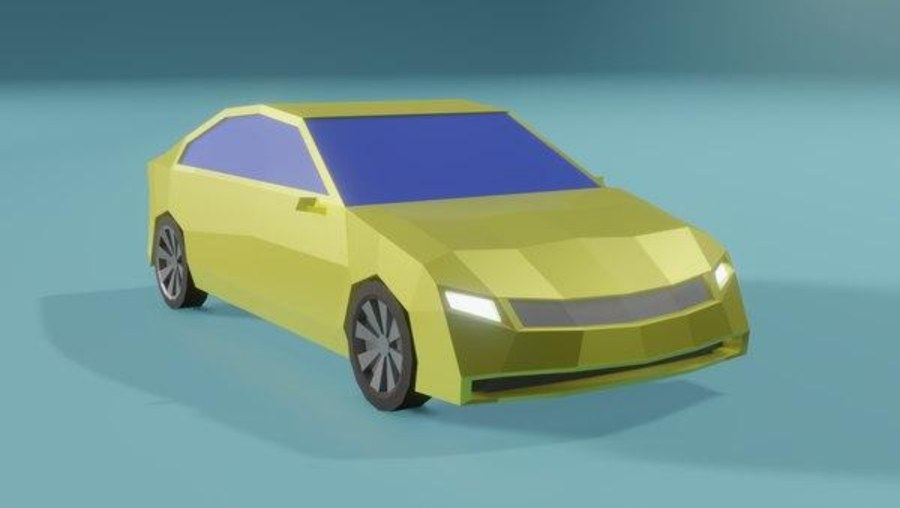
\includegraphics[width=\textwidth,height=2.6cm,keepaspectratio]{obj_voiture.jpg}\caption*{Voiture}\end{subfigure}\hfill
  \begin{subfigure}[t]{0.155\textwidth}\centering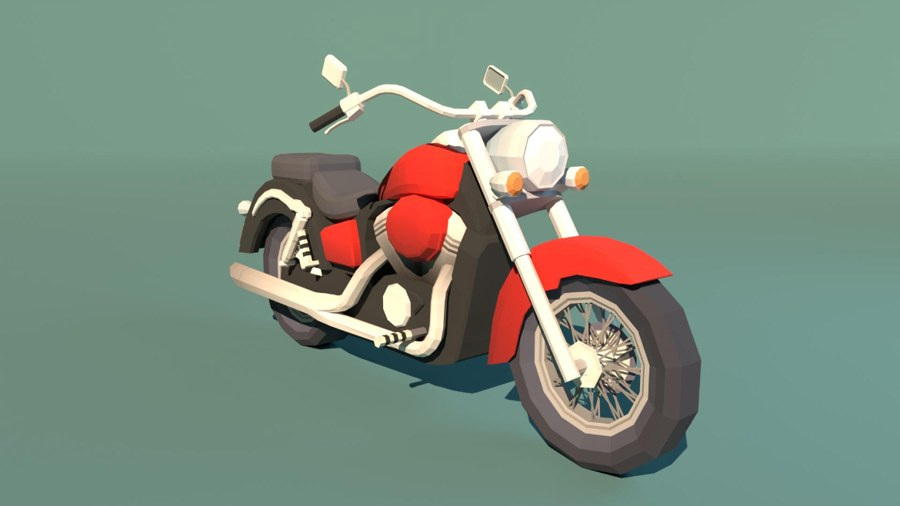
\includegraphics[width=\textwidth,height=2.6cm,keepaspectratio]{obj_moto.jpg}\caption*{Moto}\end{subfigure}\hfill
  \begin{subfigure}[t]{0.155\textwidth}\centering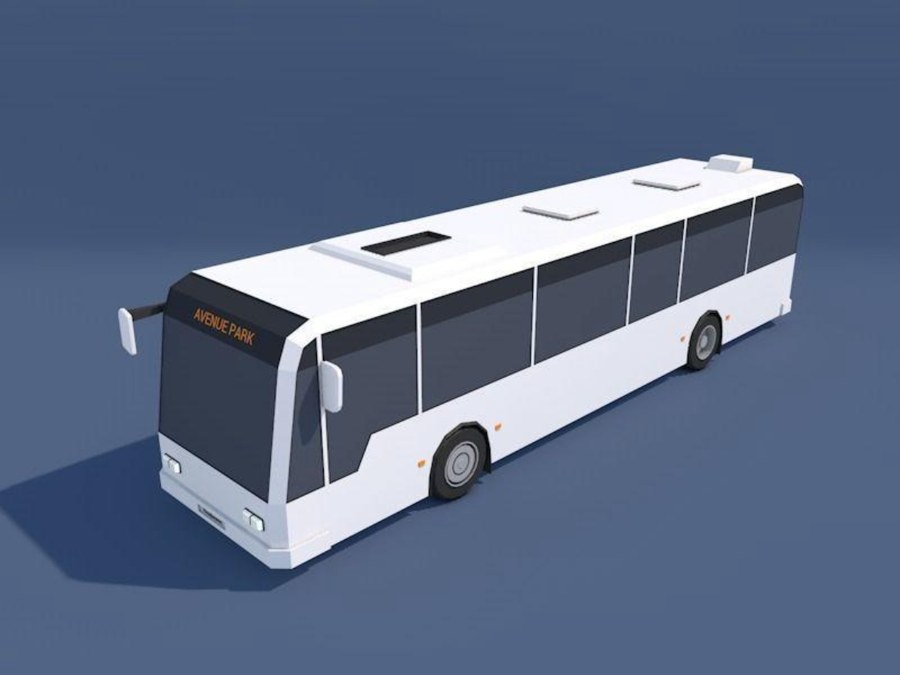
\includegraphics[width=\textwidth,height=2.6cm,keepaspectratio]{obj_bus.jpg}\caption*{Bus}\end{subfigure}\hfill
  \begin{subfigure}[t]{0.155\textwidth}\centering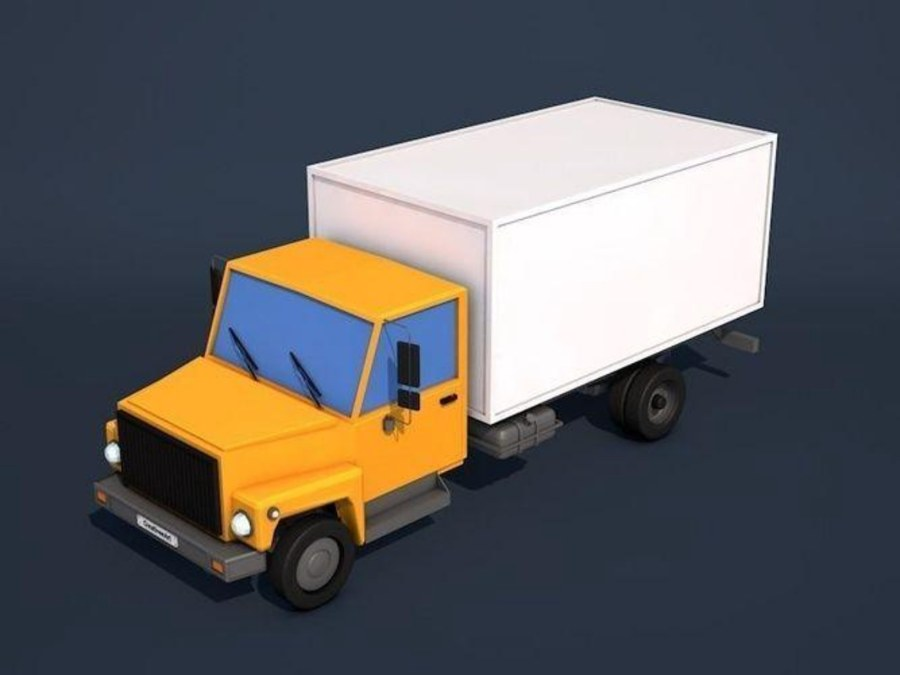
\includegraphics[width=\textwidth,height=2.6cm,keepaspectratio]{obj_camion.jpg}\caption*{Camion}\end{subfigure}
  \caption{Illustration des six classes par des modèles 3D (le modèle apprend sur des photos réelles de COCO)}
\end{figure}

\section{Analyse quantitative des données}

L'ensemble \texttt{train2017} de COCO compte \textbf{118~287 images}, dont \textbf{70~082} contiennent au moins un objet de nos classes. La résolution médiane de ces images est de 640~×~480~px.

\begin{table}[H]
\centering
\small
\caption{Nombre d'objets disponibles par classe dans COCO \texttt{train2017}}
\begin{tabular}{lrr}
  \toprule
  \entete \textbf{Classe} & \textbf{Objets annotés} & \textbf{Hors foules, plus petit côté d'au moins 32~px} \\
  \midrule
  Personne & 262~465 & 150~185 \\
  Voiture & 43~867 & 16~799 \\
  Camion & 9~973 & 7~071 \\
  Moto & 8~725 & 6~742 \\
  Vélo & 7~113 & 4~505 \\
  Bus & 6~069 & 5~194 \\
  \bottomrule
\end{tabular}
\end{table}

\begin{figure}[H]
  \centering
  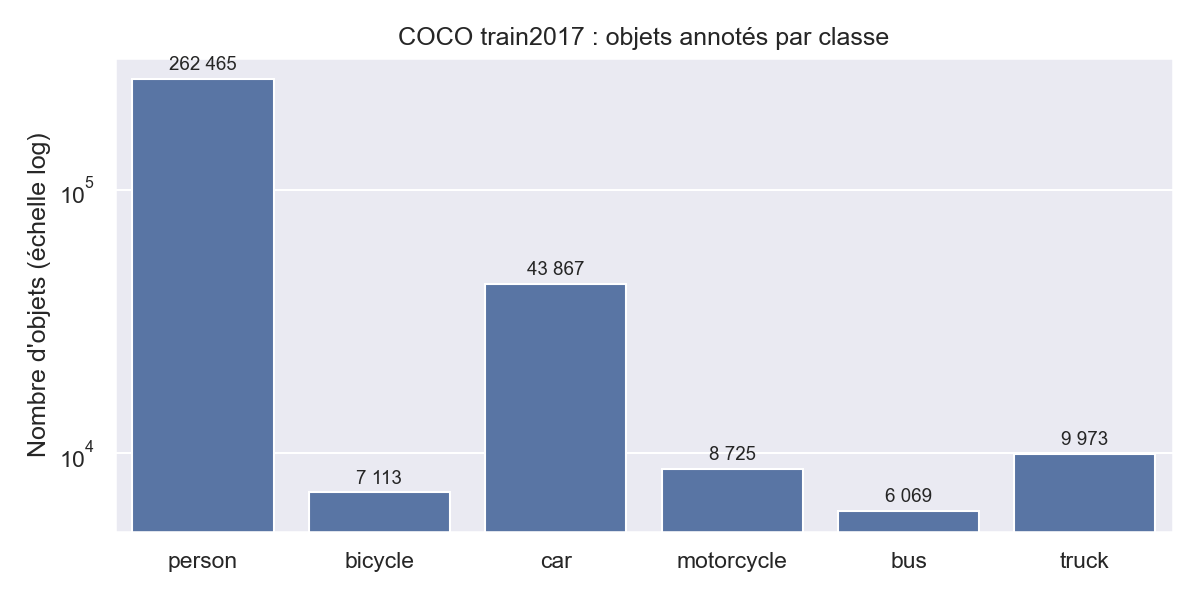
\includegraphics[width=0.66\textwidth]{01_repartition_classes.png}
  \caption{Répartition des objets par classe avant filtrage}
\end{figure}

Ces chiffres mettent en évidence un \textbf{fort déséquilibre} entre les classes : on compte 43,2 personnes pour un bus. Sans précaution, un modèle pourrait obtenir une bonne accuracy en répondant presque toujours \og personne \fg{}. C'est pourquoi nous limitons le nombre d'objets par classe et évaluons les modèles avec le F1 macro.

\section{Analyse qualitative des images}

L'observation d'exemples tirés au hasard a permis de relever plusieurs difficultés :

\begin{itemize}
  \item des objets \textbf{coupés} par le bord de la photo ou \textbf{cachés} par un autre objet ;
  \item des images \textbf{floues} ou très petites, en particulier pour les voitures éloignées ;
  \item \textbf{plusieurs objets} dans un même recadrage, comme un motard sur sa moto ;
  \item une classe \og camion \fg{} \textbf{hétérogène}, qui contient aussi des pick-ups et des camionnettes, proches d'une voiture ;
  \item des photos prises par des particuliers et non depuis un véhicule, ce qui constitue un biais à garder en tête pour un usage routier.
\end{itemize}

\section{Nettoyage des données}

Afin de ne conserver que des exemples exploitables, plusieurs règles de nettoyage ont été appliquées :

\begin{itemize}
  \item \textbf{Exclusion des foules}\\
  Une boîte marquée \texttt{iscrowd} entoure un groupe de personnes et non un seul usager.
  \item \textbf{Exclusion des petits objets}\\
  En dessous de 32~px de côté, l'objet devient trop flou une fois agrandi. À ce seuil, la classe la plus rare conserve 4~505 objets, contre seulement 2~693 avec un seuil de 64~px.
  \item \textbf{Plafond de 2~500 objets par classe}\\
  Ce plafond permet d'équilibrer les classes tout en gardant un entraînement réalisable sans GPU.
  \item \textbf{Contrôle des téléchargements}\\
  Une photo inaccessible est notée sans interrompre la préparation. Sur les 15~000 objets prévus, 14~990 ont été récupérés, 8 téléchargements ayant expiré.
\end{itemize}

\section{Redimensionnement et normalisation}

Chaque objet est découpé dans un \textbf{carré} centré sur sa boîte, avec une marge de 10~\%, puis réduit à \textbf{64~×~64~px}. Le recadrage carré évite de déformer les silhouettes, une personne étant haute et fine alors qu'un bus est large. Lorsque le carré dépasse les bords de la photo, les pixels manquants sont complétés par \textbf{reflet} plutôt que par une bande noire, que le modèle pourrait apprendre à tort.

Chaque canal de couleur est ensuite \textbf{normalisé} à l'aide de la moyenne et de l'écart-type calculés sur le jeu d'entraînement, soit [0,4057 ; 0,3894 ; 0,3748] pour la moyenne et [0,2609 ; 0,2554 ; 0,2571] pour l'écart-type. Le simulateur applique exactement les mêmes valeurs.

\begin{figure}[H]
  \centering
  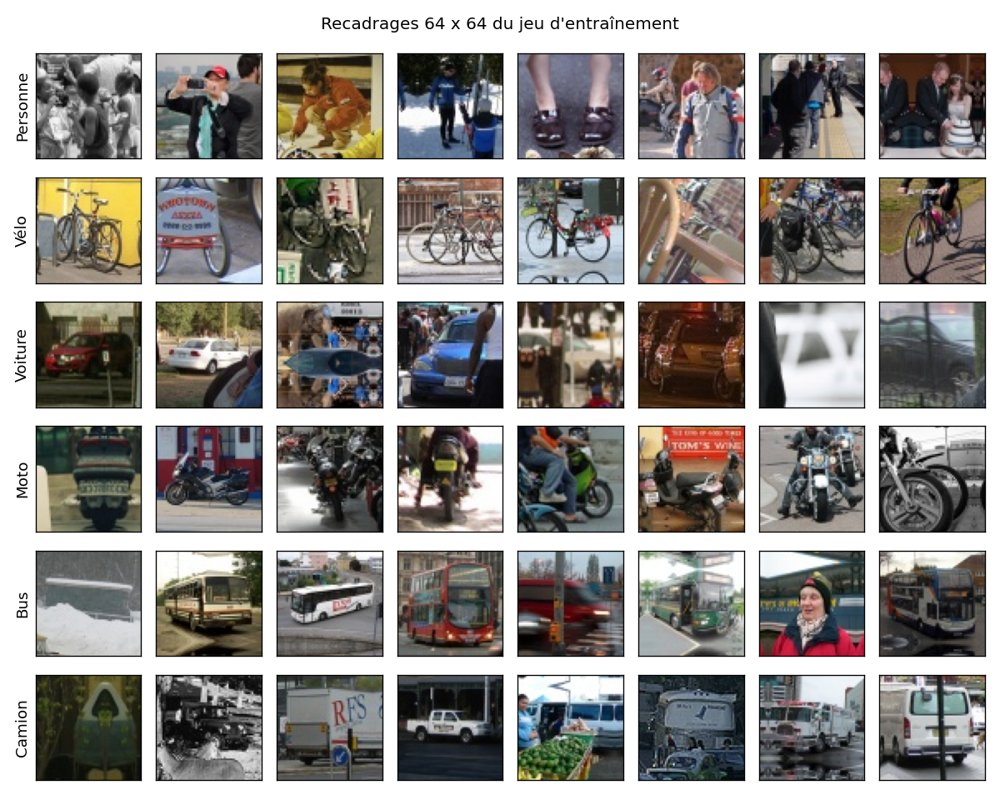
\includegraphics[width=0.58\textwidth]{02_recadrages.jpg}
  \caption{Recadrages de 64~×~64~px du jeu d'entraînement, une ligne par classe}
  \label{fig:recadrages}
\end{figure}

\section{Séparation entraînement, validation et test}

Les données ont été réparties en trois jeux : \textbf{70~\%} pour l'entraînement, \textbf{15~\%} pour la validation et \textbf{15~\%} pour le test.

\begin{table}[H]
\centering
\small
\caption{Répartition des images par classe et par jeu}
\begin{tabular}{lrrr}
  \toprule
  \entete \textbf{Classe} & \textbf{Entraînement} & \textbf{Validation} & \textbf{Test} \\
  \midrule
  Personne & 1~750 & 375 & 375 \\
  Vélo & 1~748 & 373 & 375 \\
  Voiture & 1~750 & 375 & 374 \\
  Moto & 1~750 & 374 & 375 \\
  Bus & 1~748 & 374 & 375 \\
  Camion & 1~749 & 375 & 375 \\
  \bottomrule
\end{tabular}
\end{table}

Le découpage est \textbf{stratifié}, afin de conserver les mêmes proportions de classes dans chaque jeu. Il est également réalisé \textbf{par photo d'origine}, car deux objets d'une même photo partagent le même éclairage et le même décor. Les répartir entre l'entraînement et le test fausserait donc le score. Un contrôle automatique vérifie qu'aucune des 10~672 photos n'apparaît dans deux jeux, et le découpage est enregistré dans un fichier commun afin que toute l'équipe utilise exactement les mêmes données.

\section{Conclusion}

Ce chapitre a permis de justifier le choix de \textbf{COCO 2017} et de décrire précisément les données retenues. L'analyse a mis en évidence un fort déséquilibre entre les classes ainsi que plusieurs difficultés liées à la qualité des images. Les étapes de nettoyage, de recadrage, de normalisation et de découpage par photo garantissent un jeu de données équilibré et une évaluation fiable. Ces données préparées serviront de base au modèle de classification, dont l'intégration dans l'architecture globale est détaillée dans le chapitre suivant.
